%%%%%%%%%%%%%%%%%%%%%%%%%%%%%%%%%%%%%%%%%
% Beamer Presentation
% LaTeX Template
% Version 1.0 (10/11/12)
%
% This template has been downloaded from:
% http://www.LaTeXTemplates.com
%
% License:
% CC BY-NC-SA 3.0 (http://creativecommons.org/licenses/by-nc-sa/3.0/)
%
%%%%%%%%%%%%%%%%%%%%%%%%%%%%%%%%%%%%%%%%%

%----------------------------------------------------------------------------------------
%	PACKAGES AND THEMES
%----------------------------------------------------------------------------------------

\documentclass{beamer}

\mode<presentation> {

% The Beamer class comes with a number of default slide themes
% which change the colors and layouts of slides. Below this is a list
% of all the themes, uncomment each in turn to see what they look like.

%\usetheme{default}
%\usetheme{AnnArbor}
%\usetheme{Antibes}
%\usetheme{Bergen}
%\usetheme{Berkeley}
%\usetheme{Berlin}
%\usetheme{Boadilla}
\usetheme{CambridgeUS}
%\usetheme{Copenhagen}
%\usetheme{Darmstadt}
%\usetheme{Dresden}
%\usetheme{Frankfurt}
%\usetheme{Goettingen}
%\usetheme{Hannover}
%\usetheme{Ilmenau}
%\usetheme{JuanLesPins}
%\usetheme{Luebeck}
%\usetheme{Madrid}
%\usetheme{Malmoe}
%\usetheme{Marburg}
%\usetheme{Montpellier}
%\usetheme{PaloAlto}
%\usetheme{Pittsburgh}
%\usetheme{Rochester}
%\usetheme{Singapore}
%\usetheme{Szeged}
%\usetheme{Warsaw}

% As well as themes, the Beamer class has a number of color themes
% for any slide theme. Uncomment each of these in turn to see how it
% changes the colors of your current slide theme.

%\usecolortheme{albatross}
%\usecolortheme{beaver}
%\usecolortheme{beetle}
%\usecolortheme{crane}
%\usecolortheme{dolphin}
%\usecolortheme{dove}
%\usecolortheme{fly}
%\usecolortheme{lily}
%\usecolortheme{orchid}
%\usecolortheme{rose}
%\usecolortheme{seagull}
%\usecolortheme{seahorse}
%\usecolortheme{whale}
%\usecolortheme{wolverine}

%\setbeamertemplate{footline} % To remove the footer line in all slides uncomment this line
%\setbeamertemplate{footline}[page number] % To replace the footer line in all slides with a simple slide count uncomment this line

%\setbeamertemplate{navigation symbols}{} % To remove the navigation symbols from the bottom of all slides uncomment this line
}

\usepackage{graphicx} % Allows including images
\usepackage{booktabs} % Allows the use of \toprule, \midrule and \bottomrule in tables
\usepackage[slantfont, boldfont]{xeCJK}
\usepackage{graphicx}
\usepackage{subfigure}
\usepackage{caption}
\usepackage{mathrsfs}
\usepackage{tikz}
\usetikzlibrary{decorations} 
\usetikzlibrary{decorations.pathmorphing,decorations.markings}
%----------------------------------------------------------------------------------------
%	TITLE PAGE
%----------------------------------------------------------------------------------------

\title[季调]{X13-seats季节性调整与春节节日效应} % The short title appears at the bottom of every slide, the full title is only on the title page

\author{贾昊天} % Your name
\institute[Tsinghua University] % Your institution as it will appear on the bottom of every slide, may be shorthand to save space
{
中国国际金融股份有限公司 \\ % Your institution for the title page
\medskip
\textit{Haotian.Jia@cicc.com.cn} % Your email address
}
\date{\today} % Date, can be changed to a custom date

\begin{document}

\begin{frame}
\titlepage % Print the title page as the first slide
\end{frame}

\begin{frame}
\frametitle{Overview} % Table of contents slide, comment this block out to remove it
\tableofcontents % Throughout your presentation, if you choose to use \section{} and \subsection{} commands, these will automatically be printed on this slide as an overview of your presentation
\end{frame}

%----------------------------------------------------------------------------------------
%	PRESENTATION SLIDES
%----------------------------------------------------------------------------------------

%------------------------------------------------
\begin{frame}
\frametitle{研究季调的意义}
\section{研究季调的意义} % Sections can be created in order to organize your presentation into discrete blocks, all sections and subsections are automatically printed in the table of contents as an overview of the talk
%------------------------------------------------
\begin{itemize}
\item 许多宏观经济数据存在显著的季节性与周期性,在春节时期效应尤其明显
\end{itemize}
\begin{figure}
\subfigure[出口]{
\begin{minipage}[t]{0.5\textwidth}
\centering
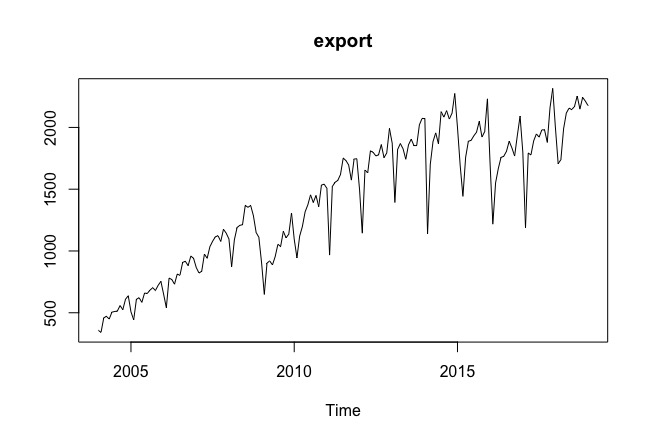
\includegraphics[width=\textwidth]{Export.jpeg}
\end{minipage}%
}\subfigure[M0]{
\begin{minipage}[t]{0.5\textwidth}
\centering
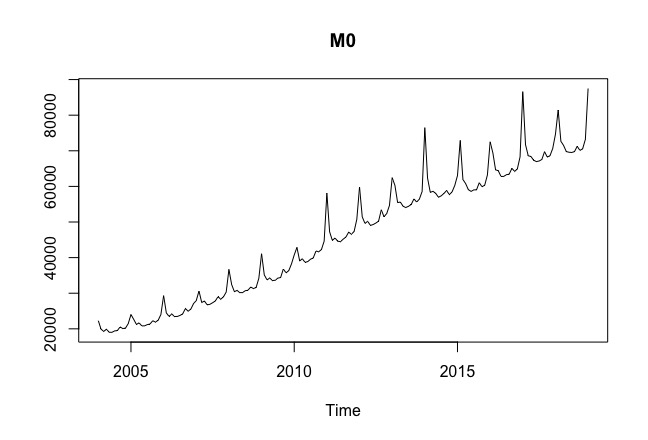
\includegraphics[width=\textwidth]{M0.jpeg}
\end{minipage}%
}
\end{figure}
\end{frame}

\begin{frame}
\frametitle{季节性调整的原理}
\section{季节性调整的原理}
\begin{itemize}
\item x-13-seats 使用的regARIMA模型,其具体的表达式如下:
\[\phi(B)\Phi(B^{s})(1-B)^{d}(1-B^{s})^{D}(y_{t}-\sum_{i}\beta_{i}x_{it})=\theta(B)\Theta(B^{s})a_{t}\]
做一个简单的变形,该模型等价于
\[(1-B)^{d}(1-B^{s})^{D}y_{t}=\sum_{i}\beta_{i}(1-B)^{d}(1-B^{s})^{D}x_{it}+w_{t}\]
\end{itemize}
\end{frame}

%------------------------------------------------

\begin{frame}
\frametitle{春节效应原理}
\section{春节效应原理}
\begin{itemize}
\item 春节效应分为节前节中和节后,数据分为流量和存量
\vskip 10pt
\begin{itemize}
\item 节前,节中节后表示春节效应的影响范围,即节前多少天,节中多少天,节后多少天的经济数据受到春节节日效应的影响
\vskip 5pt
\item 流量数据要求消除假日效应后,所得到的序列的年度总和大致等于调整之前的原序列的年度总和,存量数据的春节调整取决于当月月底是否在春节影响时效之中,不存在互补性约束
\end{itemize}
\end{itemize}
\end{frame}

%------------------------------------------------
\begin{frame}
\subsection{流量数据的春节效应}
\frametitle{流量数据的春节效应-I}
\begin{itemize}
\item 传统的季节性调整原理是对于给定月份$j$,受到节日影响的时段落在$j$月份的时间占整个受影响时段$w$的比例记为:
\[P(w,\ j)=\frac{1}{w}\text{节前(中,后)w天中落在j月份的天数}\]
\end{itemize}
\begin{center}
\pagestyle{empty}
\begin{tikzpicture}[scale=1]
\draw[->] (-5,0) -- (6,0);
\draw[red,very thick] (-3,-0.5) -- (0,-0.5);
\draw[red,very thick] (0,1) -- (2,1);
\draw[red,very thick] (2,0.3) -- (4,0.3);
\draw[dashed] (0,-0.5) -- (0,1);
\draw[dashed] (2,1) -- (2,0.3);
\draw (-1.5,-0.2) node{\tiny 节前};
\draw (1,-0.2) node{\tiny 节中};
\draw (3,-0.2) node{\tiny 节后};
\draw (-4,-0.2) node{\tiny 正常};
\draw (5,-0.2) node{\tiny 正常};
\end{tikzpicture}
\end{center}
\end{frame}
%------------------------------------------------
\begin{frame}
\frametitle{流量数据的春节效应-II}
\begin{itemize}
\item 根据栾惠德(2007),改进原模型:假设节前、节中和节后春节效应影响天数分别为$w_{b}, w_{d}, w_{a}$天,其影响强度呈线性增长,即节前第$w_{b}$天的影响权数为$\frac{1}{\sum_{i}^{w_{b}}i}$,节前第$w_{b}-1$天的影响权数为$\frac{2}{\sum_{i}^{w_{b}}i}$,$\dots$,节前第$2$天的影响权数为$\frac{w_{b}-1}{\sum_{i}^{w_{b}}i}$,节前第$1$天的影响权数为$\frac{w_{b}}{\sum_{i}^{w_{b}}i}$. 节日期间$w_{d}$天影响强度不变,节后第$1$天的影响权数为$\frac{w_{a}}{\sum_{i}^{w_{a}}i}$,节后第$2$天的影响权数为$\frac{w_{a}-1}{\sum_{i}^{w_{a}}i}$,$\dots$ , 节后第$w_{a}-1$天的影响权数为$\frac{2}{\sum_{i}^{w_{a}}i}$,节后第$w_{a}$天的影响权数为$\frac{1}{\sum_{i}^{w_{a}}i}$
\end{itemize}
\begin{center}
\pagestyle{empty}
\begin{tikzpicture}[scale=1]
\draw[->] (-5,0) -- (6,0);
\draw[red,very thick] (-3,0) -- (0,1);
\draw[red,very thick] (0,-0.5) -- (2,-0.5);
\draw[red,very thick] (2,1.5) -- (4,0);
\draw[dashed] (0,-0.5) -- (0,1);
\draw[dashed] (2,1.5) -- (2,-0.5);
\draw (-1.5,-0.2) node{\tiny 节前};
\draw (1,-0.2) node{\tiny 节中};
\draw (3,-0.2) node{\tiny 节后};
\draw (-4,-0.2) node{\tiny 正常};
\draw (5,-0.2) node{\tiny 正常};
\end{tikzpicture}
\end{center}
\end{frame}
%------------------------------------------------
\begin{frame}
\frametitle{存量数据的春节效应}
\subsection{存量数据的春节效应}
\begin{itemize}
\item 传统的存量春节效应就是当观测日落在影响期内,则定义变量为$1$,否则为$0$
\item 类似地假设节前、节中和节后春节效应影响天数分别为$w_{b}, w_{d}, w_{a}$天,假定影响呈线性增长,节前第$w_{b}$天的影响权数为$\frac{1}{w_{b}}$,节前第$w_{b}-1$天的影响权数为$\frac{2}{w_{b}}$,$\dots$,节前第$2$天的影响权数为$\frac{w_{b}-1}{w_{b}}$,节前第$1$天的影响权数为$1$. 节日期间$w_{d}$天影响强度不变,节后第$1$天的影响权数为$1$,节后第$2$天的影响权数为$\frac{w_{a}-1}{w_{a}}$,$\dots$ , 节后第$w_{a}-1$天的影响权数为$\frac{2}{w_{a}}$,节后第$w_{a}$天的影响权数为$\frac{1}{w_{a}}$
\end{itemize}
\begin{center}
\pagestyle{empty}
\begin{tikzpicture}[scale=1]
\draw[->] (-5,0) -- (6,0);
\draw[red,very thick] (-3,0) -- (0,1);
\draw[red,very thick] (0,1) -- (2,1);
\draw[red,very thick] (2,1) -- (4,0);
\draw[dashed] (0,0) -- (0,1);
\draw[dashed] (2,0) -- (2,1);
\draw (-1.5,-0.2) node{\tiny 节前};
\draw (1,-0.2) node{\tiny 节中};
\draw (3,-0.2) node{\tiny 节后};
\draw (-4,-0.2) node{\tiny 正常};
\draw (5,-0.2) node{\tiny 正常};
\end{tikzpicture}
\end{center}
\end{frame}
%---------------------------------------------
\begin{frame}
\frametitle{模型选择-I}
\section{模型选择与参数设定}
\subsection{模型选择}
\begin{itemize}
\item 季节性调整主要分为两大类:加法模型和乘法模型
\vskip 5pt
\begin{itemize}
\item 加法模型:\(Y_{t}=T_{t}+C_{t}+S_{t}+I_{t}, \quad A_{t}=T_{t}+C_{t}+I_{t}\)
\item 乘法模型:\(Y_{t}=T_{t}\times C_{t}\times S_{t}\times I_{t}, \quad A_{t}=T_{t}\times C_{t}\times I_{t}\)
\vskip 5pt
其中$Y$是原始序列,$T$是趋势因素,$C$是循环因素,$S$是季节因素,$I$是不规则因素,$A$是季调后序列
\end{itemize}
\item 对于一个时间序列,如果上述四个因素相互独立,使用加法模型更好,反之使用乘法模型更好。同时如果季节性因素规模基本保持不变,不随原始序列增长而增长,则使用加法模型;如果季节因素的规模与原始序列的水平呈比例变化,则使用乘法模型。
\item 在X13-seats包中,有自动选择模型的选项(当然也可以手动设定为加法或乘法模型)
\end{itemize}
\end{frame}
%-----------------------------------------------
\begin{frame}
\frametitle{模型选择-II}
\begin{itemize}
\item 季节性中有两个ARIMA模型需要选择:非季节性ARIMA模型和季节性ARIMA模型
\vskip 5pt
\item ARIMA(p,d,q) 模型中有三个参数$p,d,q$,分别对应模型的自回归最高阶系数(AR),差分系数,移动平均系数(MA)
\item 由regARIMA公式:\[\phi(B)\Phi(B^{s})(1-B)^{d}(1-B^{s})^{D}(y_{t}-\sum_{i}\beta_{i}x_{it})=\theta(B)\Theta(B^{s})a_{t}\]
可以选择对应的$\phi(B), \Phi(B^{s})$的最高阶系数,$d,D$的数值以及$\theta(B),\Theta(B^{s})$的最高阶系数
\item X13-seats中同样也有自动选择模型的选项
\end{itemize}
\end{frame}
%-----------------------------------------------
\begin{frame}
\frametitle{参数设定}
\subsection{参数设定}
\begin{itemize}
\item 回归有一些无法解释的特定时间点存在异常值,需要选择异常值的种类
\begin{itemize}
\item 异常值有很多种类,比如AO,LS,TC,SO等,具体的定义在manual中都有,默认有AO和LS两种异常值
\end{itemize}
\item 对于每一个数据我们需要设定不同的节前,节中以及节后天数以达到最好的模型拟合和预测结果
\item 由于Variance-Bias tradeoff, 我们需要权衡AIC,BIC等信息准则以及异常值的个数来确定最终的模型
\end{itemize}
\end{frame}
%-----------------------------------------------

\begin{frame}
\Huge{\centerline{谢谢大家}}
\end{frame}

%----------------------------------------------------------------------------------------

\end{document} 